% Mapa exponencial: álgebra de Lie → grupo de Lie
% Compilar con: pdflatex exponential_map.tex
\documentclass[tikz,border=10pt]{standalone}
\usepackage{tikz}
\usepackage{amsmath,amssymb}
\usepackage{xcolor}
\definecolor{gdlblue}{RGB}{41, 98, 168}
\definecolor{gdlred}{RGB}{191, 49, 49}
\definecolor{gdlgreen}{RGB}{30, 130, 76}
\definecolor{gdlorange}{RGB}{217, 130, 30}
\definecolor{gdlpurple}{RGB}{118, 56, 138}
\definecolor{gdlgray}{RGB}{140, 140, 140}
\definecolor{gdlyellow}{RGB}{190, 140, 10}
\usetikzlibrary{arrows.meta, positioning, decorations.pathmorphing, calc}

\begin{document}
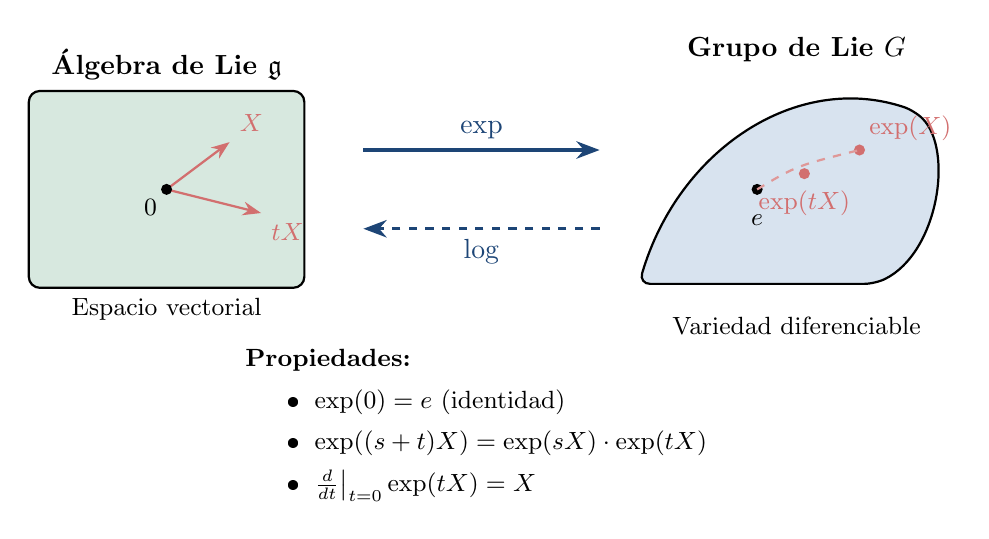
\begin{tikzpicture}[
    >=Stealth,
    space/.style={draw, thick, minimum width=3.5cm, minimum height=2.5cm, rounded corners},
    arrow/.style={->, thick, gdlblue!70!black}
]

% Álgebra de Lie (espacio tangente en la identidad)
\begin{scope}[shift={(-4,0)}]
    \node[space, fill=gdlgreen!18] (lie) {};
    \node[above] at (lie.north) {\textbf{Álgebra de Lie $\mathfrak{g}$}};
    \node[below, font=\small] at (lie.south) {Espacio vectorial};

    % Vector en el álgebra
    \draw[->, thick, gdlred!70] (lie.center) -- ++(0.8, 0.6) node[above right, font=\small] {$X$};
    \draw[->, thick, gdlred!70] (lie.center) -- ++(1.2, -0.3) node[below right, font=\small] {$tX$};

    % Origen
    \fill (lie.center) circle (2pt);
    \node[below left, font=\small] at (lie.center) {$0$};
\end{scope}

% Grupo de Lie (variedad)
\begin{scope}[shift={(4,0)}]
    % Forma curva del grupo
    \draw[thick, fill=gdlblue!18, rounded corners]
        (-2,-1.2) .. controls (-1.5,0.5) and (0,1.5) .. (1.5,1)
        .. controls (2,0.5) and (1.8,-0.8) .. (1,-1.2)
        -- cycle;
    \node[above] at (0,1.5) {\textbf{Grupo de Lie $G$}};
    \node[below, font=\small] at (0,-1.5) {Variedad diferenciable};

    % Identidad
    \fill (-0.5, 0) circle (2pt);
    \node[below, font=\small] at (-0.5,-0.2) {$e$};

    % Punto exp(X)
    \fill[gdlred!70] (0.8, 0.5) circle (2pt);
    \node[above right, font=\small, gdlred!70] at (0.8, 0.5) {$\exp(X)$};

    % Curva geodésica
    \draw[thick, gdlred!50, dashed] (-0.5, 0) .. controls (0, 0.3) .. (0.8, 0.5);

    % Punto exp(tX)
    \fill[gdlred!70] (0.1, 0.2) circle (2pt);
    \node[below, font=\small, gdlred!70] at (0.1, 0.1) {$\exp(tX)$};
\end{scope}

% Flecha del mapa exponencial
\draw[arrow, very thick] (-1.5, 0.5) -- node[above, font=\normalsize] {$\exp$} (1.5, 0.5);
\draw[arrow, very thick, dashed] (1.5, -0.5) -- node[below, font=\normalsize] {$\log$} (-1.5, -0.5);

% Propiedades
\node[font=\small, text width=6cm] at (0, -3) {
    \textbf{Propiedades:}
    \begin{itemize}
        \item $\exp(0) = e$ (identidad)
        \item $\exp((s+t)X) = \exp(sX) \cdot \exp(tX)$
        \item $\frac{d}{dt}\big|_{t=0} \exp(tX) = X$
    \end{itemize}
};

\end{tikzpicture}
\end{document}
